%%%%%%%%%%%%%%%%%%%%%%%%%%%%%%%%%%%%%%%%%%%%%%%%%%%%%%%%%%%%%%%%%%%%%%%%%%%%%%%%
%                       Hamiltonian mechanics  in maxima                       %
%                           Marc Meléndez Schofield                            %
%%%%%%%%%%%%%%%%%%%%%%%%%%%%%%%%%%%%%%%%%%%%%%%%%%%%%%%%%%%%%%%%%%%%%%%%%%%%%%%%

%%%%%%%%%%%%%%%%%%%%%%%%%%%%%%%%%%%% Head %%%%%%%%%%%%%%%%%%%%%%%%%%%%%%%%%%%%%%

\documentclass{article}
\usepackage[utf8]{inputenc}
\usepackage{amsmath}
\usepackage{comment}
\usepackage{graphicx}
\usepackage{listings}

\title{Hamiltonian mechanics in maxima}
\author{Marc Meléndez}

%%%%%%%%%%%%%%%%%%%%%%%%%%%%%%%%%%%% Body %%%%%%%%%%%%%%%%%%%%%%%%%%%%%%%%%%%%%%

\begin{document}
\maketitle

%! codeblock: introduction

This program tries to derive the Euler-Lagrange and Hamilton's canonical
equations of motion for a system described by a set of generalised coordinates
and a potential energy function. The explanation below assumes at least some
familiarity with Hamiltonian mechanics.

The maxima code written here illustrates literate programming with txt2tangle.

%! codeblockend

\section{The harmonic oscillator example}

The following code constitutes one of the simplest examples of the type of
problem that we wish to solve with our code. The point now is not that you
understand all the details in the code, but just the general idea.

We begin with a simple setup: a single mass $m$ on the $x$ axis subject to the
pull of a linear spring. Let the origin of coordinates lie at the equilibrium
point for the mass. In our one-dimensional problem, we need only one coordinate
($q$) to describe the position of the mass. Therefore, our code begins with

\lstset{morecomment = [is]{\%!}{\^^M}}
\begin{lstlisting}[frame=single]
%! codefile: harmonic.mc
dim: 1; /* Dimensionality */
M: 1; /* Number of bodies */
N: 1; /* Number of degrees of freedom */
%! codepause
\end{lstlisting}

The elastic energy in the spring equals
\begin{equation*}
  V(q) = \frac{1}{2} k q^2,
\end{equation*}
where $k > 0$ stands for the spring constant.
\begin{lstlisting}[frame=single]
%! codecontinue: harmonic.mc
/* Potential energy */
assume(k > 0);
V(q, qdot, t) := (k/2)*q[1]^2;
%! codepause
\end{lstlisting}
Next, we need to define the relation between generalised coordinates and
cartesian coordinates. In this case, our coordinate $q$ is simply the
$x$ coordinate.
\begin{lstlisting}[frame=single]
%! codecontinue: harmonic.mc
/* Position of the system set by the x coordinate */
r[1, 1](q, t) := q[1];
%! codepause
\end{lstlisting}

In section \ref{Euler-Lagrange_equations}, we will write the maxima script
\texttt{eqmotion.mc}, which derives the equations of motion for a system defined
as above.
\begin{lstlisting}[frame=single]
%! codecontinue: harmonic.mc
/* Determine the equations of motion */
load("eqmotion.mc");
%! codepause
\end{lstlisting}
Following the execution of this script, we can print the Euler-Lagrange
equation of motion:
\begin{lstlisting}[frame=single]
%! codecontinue: harmonic.mc
/* Output the Euler-Lagrange equation of motion
   (Netwon's second law) */
display(EulerLagrange[1]);
%! codepause
\end{lstlisting}
For the harmonic oscillator,
\begin{equation*}
  m \frac{d^2 q}{dt^2} + k q = 0,
\end{equation*}
rendered in maxima as

\begin{minipage}{\textwidth}
\begin{verbatim}
           2
          d
      m  (--- (q (t))) + k q (t) = 0
       1    2   1           1
          dt
\end{verbatim}
\end{minipage}

Following this, we could output the Hamilton's equations with
\begin{lstlisting}[frame=single]
%! codecontinue: harmonic.mc
/* Output Hamilton's equations of motion */
display(Hamilton[1][1]);
display(Hamilton[1][2]);
%! codepause
\end{lstlisting}
For our mass-on-a-spring system, the equations read
\begin{align*}
  \frac{dq}{dt} & = \frac{p}{m}, \\
  \frac{dp}{dt} & = -k q.
\end{align*}
which come out in maxima as

\begin{minipage}{\textwidth}
\begin{verbatim}
                   p
      d             1
      -- (q (t)) = --
      dt   1       m
                    1
      d
      -- (p (t)) = - q  k
      dt   1          1
\end{verbatim}
\end{minipage}

Once we have the equations of motion, we can try to solve them or use them to
set up numerical simulations. For example, the harmonic oscillator code could
end with
\begin{lstlisting}[frame=single]
%! codecontinue: harmonic.mc
/* Solve differential equation */
ode2(EulerLagrange[1], q[1](t), t);
%! codeend
\end{lstlisting}
Executing the program (\texttt{maxima -b harmonic.mc}) from the command line
will end up giving you the formula for the motion of the particle:

\begin{minipage}{\textwidth}
\begin{verbatim}
                      sqrt(k) t            sqrt(k) t
      q (t) = %k1 sin(---------) + %k2 cos(---------)
       1              sqrt(m )             sqrt(m )
                            1                    1
\end{verbatim}
\end{minipage}

\section{Interacting particles}

Suppose that instead of a single particle, we have two masses on the $x$ axis
attached by a spring. In that case, the potential energy would equal
\begin{equation*}
  V(q_1, q_2) = \frac{1}{2} k (q_2 - q_1)^2.
\end{equation*}
which in code reads
\begin{lstlisting}[frame=single]
%! codefile: two_springs.mc
/* Potential energy */
assume(k > 0);
V(q, qdot, t) := (k/2)*(q[2] - q[1])^2;
%! codepause
\end{lstlisting}
Even though \textit{this} particular potential energy function is independent of
the generalised velocities ($\dot{q}$, \texttt{qdot} in the code) and time, we
leave open the possibility for other functions that do depend on velocities or
time. We assume that we still have a one-dimensional problem. In this case,
though, we have two coordinates (degrees of freedom) corresponding to the two
masses. \begin{lstlisting}[frame=single]
%! codecontinue: two_springs.mc
dim: 1; /* Dimensionality */
M: 2; /* Number of bodies */
N: 2; /* Number of degrees of freedom */
%! codepause
\end{lstlisting}
We indicate that the coordinates correspond to $x$ coordinates of masses one and
two. In the relation between cartesian and generalised coordinates
\texttt{r[i,j]} ($r_{ij}$) stands for the $j$th coordinate of particle number
$i$.
\begin{lstlisting}[frame=single]
%! codecontinue: two_springs.mc
r[1, 1](q, t) := q[1];
r[2, 1](q, t) := q[2];
%! codeinsert: get_equations
%! codepause
\end{lstlisting}
After these definitions, we could simply load \texttt{eqmotion.c} again and then
print out the equations of motion.
\begin{lstlisting}[frame=single]
%! codeblock: get_equations
/* Determine the equations of motion */
load("eqmotion.mc");

display("Euler-Lagrange equations:");
for i: 1 thru N do
  display(EulerLagrange[i]);

display("Hamilton's equations:");
for i: 1 thru N do (
    display(Hamilton[i][1]),
    display(Hamilton[i][2])
);
%! codeblockend
\end{lstlisting}
Running the script would produce the equations of motion. The Euler-Lagrange
equations, for example, come out as
\begin{equation*}
  m_i \frac{d^2 q_i}{dt^2} + k(q_i - q_j) = 0,\ i \neq j.
\end{equation*}

\section{Generalised coordinates}

Alternatively, we might wish to represent the dynamics of these two masses in
terms of the position of the centre of mass and the coordinate difference,
that is,
\begin{align*}
  q_1 & = \frac{m_1 x_1 + m_2 x_2}{m_1 + m_2}, \\
  q_2 & = x_2 - x_1.
\end{align*}
Solving for $x_1$ and $x_2$,
\begin{align*}
  x_1 & = q_1 - \frac{m_2}{m_1 + m_2} q_2, \\
  x_2 & = q_1 + \frac{m_1}{m_1 + m_2} q_2.
\end{align*}
Then we would write
\begin{lstlisting}[frame=single]
%! codefile: normal_modes.mc
dim: 1; /* Dimensionality */
M: 2; /* Number of bodies */
N: 2; /* Number of degrees of freedom */

r[1, 1](q, t) := q[1] - m[2]*q[2]/(m[1] + m[2]);
r[2, 1](q, t) := q[1] + m[1]*q[2]/(m[1] + m[2]);

/* Potential energy */
assume(k > 0);
V(q, qdot, t) := (k/2)*q[2]^2;
%!
%! codeinsert: get_equations
%! codeend
\end{lstlisting}
When maxima derives the canonical equations, we get decoupled differential
equations for the new coordinates (normal modes).
\begin{align*}
  \frac{dq_1}{dt} = \frac{p_1}{m_1 + m_2},\  &
  \ \frac{dp_1}{dt} = 0, \\
  \frac{dq_2}{dt} = \frac{(m_1 + m_2) p_2}{m_1 m_2},\  &
  \ \frac{dp_2}{dt} = -k q_2.
\end{align*}

The simple pendulum of length $l$ and mass $m$ serves as a basic example
defining generalised coordinates that does not involve cartesian coordinates.
Here we have a single angle coordinate (represented by $q_1$), but motion on the
$xy$ plane. The gravitational potential energy equals mass times gravitational
acceleration times height,
\begin{equation*}
  V(q_1) = m g l(1 - \cos(q_1)),
\end{equation*}
and the relation between the angle and the coordinates is
\begin{align*}
  x = l \sin(q_1), \\
  y = l (1 - \cos(q_1)).
\end{align*}
In maxima code, we write
\begin{lstlisting}[frame=single]
%! codefile: pendulum.mc
dim: 2; /* Dimensionality */
M: 1; /* Number of bodies */
N: 1; /* Number of degrees of freedom */

r[1, 1](q, t) := l*sin(q[1]);
r[1, 2](q, t) := l*(1 - cos(q[1]));

/* Potential energy */
V(q, qdot, t) := m[1]*g*l*(1 - cos(q[1]));
%!
%! codeinsert: get_equations
%! codeend
\end{lstlisting}
Then we load \texttt{eqmotion.mc} to calculate the equations of motion
for the pendulum, as in the examples above.

\section{\label{Euler-Lagrange_equations}Derivation of the Euler-Lagrange 
equations of motion}

An educational code that achieves the effects showcased above, at least in
simple cases, requires no great performance of programming wizardry. Rather, we
will simply follow the standard steps of classical Hamiltonian mechanics.

To construct the Lagrangian function, which depends on the generalised
coordinates $q_i$ and velocities $\frac{dq_i}{dt} = \dot{q}_i$, as well as
(possibly) time $t$,
\begin{equation}
\label{Lagrangian}
  L(\mathbf{q}, \dot{\mathbf{q}}, t)
   = T(\mathbf{q}, \dot{\mathbf{q}}, t) - V(\mathbf{q}, \dot{\mathbf{q}}, t),
\end{equation}
we need the kinetic and potential energy functions, $T$ and $V$. We have already
seen how to write the potential energy $V$. We define $T(q, \dot{q}, t)$ as
\begin{equation}
\label{kinetic_energy}
  T(\mathbf{q}, \dot{\mathbf{q}}, t)
    = \sum_{i = 1}^M\sum_{j = 1}^{d} \frac{1}{2} m_i \dot{r}_{ij}^2.
\end{equation}
Here, $d$ represents the system dimensionality (\texttt{dim} in the code).
\begin{lstlisting}[frame=single]
%! codeblock: kinetic_energy
/* Kinetic energy */
for i: 1 thru M do assume(m[i] > 0);
T(q, qdot, t)
  := trigsimp(
       sum((m[i]/2)
           *sum((rdot[i, j](q, qdot, t))^2, j, 1, dim),
           i, 1, M)
     );
%! codeblockend
\end{lstlisting}
The extra \texttt{trigsimp} was added just to simplify some of the expressions.
The \texttt{rdot[i,j]} ($\dot{r}_{ij}$) stand for the cartesian
velocity coordinates, which we calculate as
\begin{equation}
  \dot{r}_{ij}
    = \sum_{k = 1}^N \frac{\partial r_{ij}}{\partial q_k}\dot{q}_k
      + \frac{\partial r_{ij}}{\partial t}.
\end{equation}
\begin{lstlisting}[frame=single]
%! codeblock: velocities
/* Velocities */
for i: 1 thru M do (
  for j: 1 thru dim do (
    rdot[i, j](q, qdot, t)
      := sum(diff(r[i, j](q, t), q[k])
             *qdot[k], k, 1, N)
         + diff(r[i, j](q, t), t)
  )
);
%! codeblockend
\end{lstlisting}

We can now define the Lagrangian function (\ref{Lagrangian}) by subtracting the
potential energy $V$ from the kinetic energy (\ref{kinetic_energy}).
\begin{lstlisting}[frame=single]
%! codeblock: Lagrangian
/* Lagrangian */
L(q, qdot, t) := T(q, qdot, t) - V(q, qdot, t);
%! codeblockend
\end{lstlisting}
The Euler-Lagrange equations of motion emerge from the Lagrangian by working out
\begin{equation}
  \frac{d}{dt}\left(\frac{\partial}{\partial \dot{q}_i}\right)
  - \frac{\partial L}{\partial q_i} = 0
\end{equation}
\begin{lstlisting}[frame=single]
%! codeblock: EulerLagrange
/* Euler-Lagrange equations of motion */
for i: 1 thru N do
EulerLagrange[i]:
  diff(subst(diff(q[i](t), t), qdot[i],
             diff(L(q, qdot, t), qdot[i])), t)
  -subst(q[i](t), q[i],
             diff(L(q, qdot, t), q[i])) = 0;
%! codeblockend
\end{lstlisting}
Where the \texttt{subst} function substitutes $q_i(t)$ for $q_i$ to indicate
explicitly that the coordinates are functions of time.

\section{Hamilton's canonical equations}

To calculate the canonical equations of motion, we need to write the Hamiltonian
function, which arises as a Legendre transform of the Lagrangian.
\begin{equation}
\label{Hamiltonian}
  H(\mathbf{q}, \mathbf{p}, t)
    = \sum_{k = 1}^N \dot{q}_i p_i - L(q, \dot{q}_i, t).
\end{equation}
The $p_i$ represent the generalised conjugate momenta. In order to write the
definition in terms of the right variables, we need to express the generalised
velocities $\dot{q}_i$ as a function of the $p_i$. From the definition of $p_i$
\begin{equation}
  p_i = \frac{\partial L}{\partial \dot{q}_i},
\end{equation}
we obtain a system of equations, which we then solve for the $\dot{q}_i$. In the
code below, we use the variable \texttt{v[i]} to represent $\dot{q}_i$ expressed
in terms of the momenta $p_i$.
\begin{lstlisting}[frame=single]
%! codeblock: generalised_momenta
/* Generalised momenta */
momentum_equations: []; momentum_variables: [];
for i: 1 thru N do (
  momentum_equations:
    append(momentum_equations,
           [p[i] = diff(L(q, qdot, t), qdot[i])]),
  momentum_variables:
    append(momentum_variables, [qdot[i]])
);

momentum_solutions:
  solve(momentum_equations, momentum_variables);

if N = 1
  then v[1]: rhs(momentum_solutions[1])
else
  for i: 1 thru N do
    v[i]: rhs(momentum_solutions[1][i]);
%! codeblockend
\end{lstlisting}
The special case for one degree of freedom $N = 1$ appears because maxima
provides the solution in a different format when it solves for a system of
equations and several variables (a list of lists as opposed to a list).

Now we can write the Hamiltonian (\ref{Hamiltonian}),
\begin{lstlisting}[frame=single]
%! codeblock: Hamiltonian
/* Hamiltonian */
H(q, p, t)
  := expand(sum(p[i]*v[i], i, 1, N) - L(q, v, t));
%! codeblockend
\end{lstlisting}
from which the canonical equations result by writing
\begin{align}
  \dot{q}_i & = \frac{\partial H}{\partial p_i}, \\
  \dot{p}_i & = -\frac{\partial H}{\partial q_i},
\end{align}
where $\dot{p}_i$ stands for the time derivative of $p_i$. These equations give 
us the final lines of code.
\begin{lstlisting}[frame=single]
%! codeblock: canonical
/* Hamilton's canonical equations */
for i: 1 thru N do
  Hamilton[i]:
    [diff(q[i](t), t)
       = trigsimp(diff(H(q, p, t), p[i])),
     diff(p[i](t), t)
       = -trigsimp(diff(H(q, p, t), q[i]))];
%! codeblockend
\end{lstlisting}

\begin{comment}
Putting all the pieces together, the final code has the following structure:
%! codefile: eqmotion.mc

%! codeinsert: velocities

%! codeinsert: kinetic_energy

%! codeinsert: Lagrangian

%! codeinsert: EulerLagrange

%! codeinsert: generalised_momenta

%! codeinsert: Hamiltonian

%! codeinsert: canonical

%! codeend
\end{comment}

\section{Numerical simulation}

The equations of motion give us the power to set up simple numerical
simulations. Now, in that case, we must remember to specify the values of all
the numerical parameters. For example, for a double pendulum (Figure
\ref{double_pendulum}) we would need to assign the values of the lengths $l_1$
and $l_2$, both masses and the acceleration of gravity, $g$.
\begin{lstlisting}[frame=single]
%! codefile: double_pendulum.mc
/* System parameters */
dim: 2; M: 2; N: 2;
l[1]: 1; l[2]: 1; m[1]: 1; m[2]: 1; g: 9.8;
%! codepause
\end{lstlisting}

\begin{figure}
  \centering
  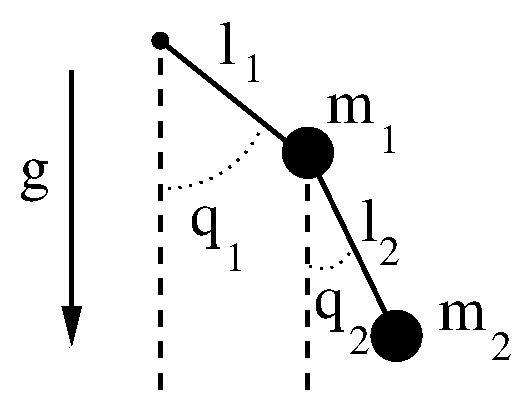
\includegraphics[width = 0.5 \textwidth]{double_pendulum.eps}
  \caption{\label{double_pendulum}Parameters in the double pendulum. The 
                  generalised coordinates $q_1$ and $q_2$ represent the
                  angles with the vertical directions, the masses are $m_i$, 
                  the lenghts $l_i$ and the acceleration of gravity is $g$.}
\end{figure}

Then, as usual, we would just write down the transformation from generalised
coordinates to cartesian coordinates, the potential energy, and follow these
lines with the calculation of the equations of motion by calling
\texttt{eqmotion.mc}.
\begin{lstlisting}[frame=single]
%! codecontinue: double_pendulum.mc
/* Coordinates */
r[1,1](q, t) := l[1]*sin(q[1]);
r[1,2](q, t) := l[1] + l[2] - l[1]*cos(q[1]);
r[2,1](q, t) := r[1,2](q, t) + l[2]*sin(q[2]);
r[2,2](q, t) := r[1,1](q, t) - l[2]*cos(q[2]);

/* Potential energy */
V(q, qdot, t)
  := m[1]*g*r[1,2](q, t) + m[2]*g*r[2,2](q, t);

/* Equations of motion */
load("eqmotion.mc");
%! codepause
\end{lstlisting}
The following lines of code should work like this: we set the time step, number
of steps and sampling (how many steps to next data output), and the name of the
output file. Then we provide initial conditions and run the sumulation by
calling \texttt{Euler.mc}. We use $\mathbf{z}$ as a shorthand notation for the
state of the system.
\begin{equation}
  \mathbf{z}(t) = (q_1(t), p_1(t), q_2(t), p_2(t), \ldots, q_N(t), p_N(t)),
\end{equation}
so we initialise the system with a list of coordinate and momentum values.
\begin{lstlisting}[frame=single]
%! codecontinue: double_pendulum.mc
/* Simulation parameters */
dt: 0.001; nsteps: 10000; sampling: 100;

/* Output file */
EulerOutput: openw("double_pendulum.dat");

/* Initial conditions */
z:[0.75, 0, 0.7, 0];

/* Numerical simulation */
load("Euler.mc");
%! codeend
\end{lstlisting}
The \texttt{Euler.mc} code moves the sistem in time by advancing in small steps.
\begin{align}
  \Delta q_i & = \frac{\partial q_i}{\partial t} \Delta t, \\
  \Delta p_i & = \frac{\partial p_i}{\partial t} \Delta t. \\
\end{align}
Of course, the canonical equations give us the formula for the time derivatives.
\begin{align}
  \Delta q_i & = \frac{\partial H}{\partial p_i} \Delta t, \\
  \Delta p_i & = -\frac{\partial H}{\partial q_i} \Delta t. \\
\end{align}
The \texttt{Euler.mc} code then outputs rows listing the time, followed by the
elements of $\mathbf{z}$ and ending with the value of the Hamiltonian function
for that state.

We achieve this effect by writing two paragraphs of code in \texttt{Euler.mc},
the first of which calculates the analytical expression of $\Delta z$.
\begin{lstlisting}[frame=single]
%! codefile: Euler.mc
/* Build expressions for Delta z */
Deltaz: [];
for i: 1 thru N do (
  Deltaz:
    append(Deltaz, rhs(Hamilton[i][1])*dt),
  Deltaz:
    append(Deltaz, rhs(Hamilton[i][2])*dt)
);
%! codepause
\end{lstlisting}
The final paragraph inserts the current coordinate and momenta values of the 
system into $\Delta z$ to calculate the new state, and repeats this process 
\texttt{nsteps} times. We do this in two steps. First, we construct a list of 
variables and their values (for example, $[q_1 = 1, p_1 = 0, \ldots, q_N = 0.5, 
p_N = 1, t = 0]$). Then we calculate $\Delta z$ at these values and add it to 
the current coordinate values to get the new position.
\begin{lstlisting}[frame=single]
%! codecontinue: Euler.mc
/* Integrate the equations of motion (Euler scheme) */
for step: 1 thru nsteps do (
  for i: 1 thru N do (
    z0:
      append(z0, [q[i] = z[2*i - 1]]),
    z0:
      append(z0, [p[i] = z[2*i]]),
  ),
  z0: append(z0, [t = stp*dt]),
  z: at(z + Deltaz, z0),
  if mod(step, sampling) == 0 then (
    printf("~f", step*dt),
    for i: 1 thru N do
      printf(EulerOutput, " ~f ~f", z[2*i - 1], z[2*i]),
    printf(" ~f~%", at(H(q, p, t), z0))
  )
);
%! codeend
\end{lstlisting}
At the end, we output time, state and total energy (Hamiltonian function) at the 
right time steps.

\end{document}

%! codefile: README.md
# Hamiltonian mechanics in maxima

%! codeinsert: introduction
%! codeend

%! codefile: Makefile
all: code weave

code:
	txt2tangle mechanics.tex

weave:
	latex mechanics.tex
	dvips mechanics.dvi
	ps2pdf mechanics.ps
%! codeend
